%NOTE: This doc formatted according to http://ec.europa.eu/research/participants/data/ref/h2020/call_ptef/pt/2018-2020/h2020-call-pt-erc-stg-2019_en.pdf

\documentclass[11pt,a4paper]{article}
\usepackage[left=2.0cm,top=2.0cm,right=2.0cm,bottom=1.5cm]{geometry}               
%\usepackage[subtle]{savetrees}
\usepackage[bibbreaks=normal, paragraphs=normal, floats=tight, mathspacing=tight, lists=tight, title=normal, margins=normal, wordspacing=normal, tracking=normal, charwidths=normal, bibnotes=normal, mathdisplays=tight, leading=normal, indent=normal, bibliography=tight, sections=tight]{savetrees} 

\usepackage{graphicx}
\usepackage{amssymb}
\usepackage{epstopdf}
\usepackage{xspace}     
\usepackage{wrapfig}
\setlength\intextsep{0pt}

\usepackage{color}
\usepackage{colortbl}
\usepackage{amsmath} % Adds a large collection of math symbols                  
\usepackage{ifthen} % for conditional statements               
\usepackage{amssymb}
\usepackage{amsfonts}
\usepackage{upgreek} % Adds in support for greek letters in roman typeset       
\usepackage{titling}
\usepackage{makecell}
\usepackage{pgfgantt}
\usepackage{lscape}
\usepackage{multirow}
\usepackage{titlesec}
\usepackage{url,booktabs,amsmath,hepunits,abhepexpt,abhep,xcolor}%amsmath
\usepackage[colorlinks]{hyperref}    % Hyperlinks in references
\usepackage[all]{hypcap} % Internal hyperlinks to floats.

\newboolean{uprightparticles}
\setboolean{uprightparticles}{false} %Set to true to get roman particle symbols

%If we need more space we can investigate: https://tex.stackexchange.com/questions/273086/use-smaller-headheight-in-fancyhdr, https://tex.stackexchange.com/questions/271159/turn-off-fancyhdr-auto-spacing
\usepackage{fancyhdr}

\usepackage{rotating}

%\usepackage{fancyheadings}
\pagestyle{fancy}


% Playing with the page size 

\usepackage{array}
\newcolumntype{y}[1]{>{\raggedleft\arraybackslash}p{#1}}

%\renewcommand*{\arraystretch}{1.2}

%TB
%\addtolength{\oddsidemargin}{-10pt}
%\addtolength{\evensidemargin}{-10pt}
%\addtolength{\textwidth}{25pt}
%\addtolength{\textheight}{76pt}
%end TB

%\addtolength{\textfloatsep}{-2pt}
\setlength{\droptitle}{-44mm}

\setlength{\headwidth}{\textwidth}


\newboolean{articletitles}
\setboolean{articletitles}{false}

\usepackage{cite}
\usepackage{mciteplus}

\newboolean{inbibliography}

\titlespacing{\section}{0pt}{4pt}{0pt}
\titlespacing{\subsection}{0pt}{4pt}{0pt}
\titlespacing{\subsubsection}{0pt}{4pt}{0pt}

%\titlespacing{\section}{0pt}{\parskip}{0pt}
%\titlespacing{\subsection}{0pt}{\parskip}{0pt}
%\titlespacing{\subsubsection}{0pt}{\parskip}{0pt}

%Garamond saves space and looks way poncier
%\usepackage[T1]{fontenc}
%\usepackage[urw-garamond]{mathdesign}
\usepackage{ebgaramond}
\renewcommand\labelitemi{$\bullet$}


\usepackage{fontspec}

\setmainfont{EBGaramond-Regular}[
  BoldFont = EBGaramond-Bold,
  ItalicFont = EBGaramond-Italic,
  BoldItalicFont = EBGaramond-BoldItalic]
  
%\usepackage[cmintegrals,cmbraces]{newtxmath}
%\usepackage{ebgaramond-maths}
%\usepackage[T1]{fontenc}

% Helvetica for sans serif
% (scaled to match size of Palatino)
%\usepackage[scaled=0.90]{helvet}
%\usepackage{helvet}

\title{{\Large Part B1 - ERC Consolidator grant}}
\author{{\normalsize Caterina Doglioni}}
\date{}                                           % Activate to display a given date or no date

\usepackage[parfill]{parskip}
%\setlength{\parskip}{0.5em}


\begin{document}
\lhead{{\small Doglioni}}
\chead{{\small Part B1}}
\rhead{{\small REALDARK}}
\begin{center} 

{\Large\bf ERC Consolidator Grant 2020} \\
	{\Large\bf Research Proposal [Part B1]}  \\
 
\vspace{2cm} 
{\huge {\bf }}   \smallskip  

\vspace{2cm} 
{\Huge{REALDARK}} \\
\medskip  
{\large{REAL-time discovery strategies for DARK matter and dark sector signals \\ at the ATLAS detector with Run-3 LHC data}} \\ 

\vspace{1cm} 
\vspace{1cm}
\end{center} 
\begin{tabular}{rcl}
Principal Investigator & : & Dr.~Caterina~Doglioni \\
Host Institution & : & Lund University \\ 
Proposal duration in months & : & 60 \\
\end{tabular}  
\vspace{2cm}


\begin{center} {\bf Summary}  \end{center}

%Old abstract
%The Standard Model of Particle Physics (SM) describes the fundamental particles and interactions of ordinary matter. Despite the SM's success in predicting experimental results, it fails to account for the large excess of unobservable (Dark) matter in the Universe. 
%A compelling hypothesis is that Dark Matter (DM) particles can be created from SM particle collisions, such as those produced by the Large Hadron Collider and recorded by the experiments at the CERN laboratory. 
%%Tim's comment: "compelling" probably OK in the abstract, but make sure you convince the reader in the main proposal that it is really compelling
%
%In the \textsc{Realdark} project, I will consolidate my leadership in dark matter searches with innovative data-taking techniques, with a team of postdoctoral researchers and students at Lund University working on the ATLAS experiment. 
%
%%Oxana: Expand on real-time analysis and why this is novel (wait for AB's comments to do this)
%This research program makes use of real-time data analysis techniques to make the most of the vast amount of LHC data collected by the ATLAS experiment, 
%%Oxana doesn't like "resource-constrained" as it's not clear where it's coming from
%expanding the ATLAS physics program in a resource-constrained, data-rich environment. 
%The technical outcomes of \textsc{Realdark} will be shared with the wider community, providing valuable input towards technological advancements. 
%
%%Following was edited from "extend and deploy" following Tim's comment that it sounds like I'm doing the same thing over
%Relying on preliminary results achieved within my ERC Starting Grant \textsc{Darkjets}, within this project we will deliver new ways of taking data, 
%and exploit the datasets recorded in the upcoming LHC data-taking period to search for evidence of processes related to dark matter. 
%We will pursue broad searches for dark matter models that theorize weakly interacting massive particles and dark sector particles at a crucial time for the global quest for dark matter. 
%The outcomes of this project will define the direction of future experiments and theoretical efforts: 
%The planned searches will yield either a discovery of a dark matter particle candidate ready to study in connection with astrophysical observations, or constraints on the particle nature of dark matter. 

The Standard Model of Particle Physics (SM) describes the fundamental particles and interactions of ordinary matter. Despite the SM's success in predicting experimental results, it fails to account for the large abundance of dark matter in the Universe. 
Dark Matter (DM) particles could be created from collisions of SM particles, such as in the Large Hadron Collider, but storage and computing limitations mean that rare processes involving DM may be missed by current data taking methods. 

In \textsc{Realdark}, I will consolidate my leadership in DM searches with innovative data-taking techniques that solve this problem for the ATLAS experiment. The technical innovations of \textsc{Realdark} will be disseminated, paving the way to advancements for future experiments.

Under my leadership, the \textsc{RealDark} team will break the traditional paradigm of recording detector data and then analyzing it in separate steps, by deploying data processing in real-time so that far more collision data can be searched for rare processes. 
We will enable new types of datasets from the upcoming LHC data-taking period and search them for new phenomena, motivated by theories of weakly interacting massive DM particle candidates and particles from a \textit{dark} sector inaccessible to ordinary particles. 

The proposed searches will yield either a discovery of dark matter candidates, to be studied in connection with astrophysical observations, or world-leading constraints on the particle nature of dark matter, focusing theoretical efforts and search targets for future experiments.  

\clearpage

\section*{Section A: Extended synopsis of the proposal} 

\medskip

\section{Aims and impact of this research project} 
\smallskip

% problem
% what you are going to do
% followed by who you are
% followed by the longer term impact
% end intro section

The first years of data-taking at the Large Hadron Collider (LHC)~\cite{LHC2008} at CERN yielded the discovery of a new fundamental particle, the Higgs boson~\cite{Khachatryan:2016vau}. With this and many other notable results, the LHC has confirmed the Standard Model (SM) of particle physics, the theory of fundamental particles and the non-gravitational interactions among them. 
However, astrophysical observations show the amount of matter described by the SM is exceeded by a factor of five by another kind of matter called Dark Matter (DM)~\cite{Bertone:2016nfn}. 

Many theoretical models explain the abundance of DM in the universe using particles that interact weakly with the SM, called WIMPs. 
If produced by the LHC, their discovery could complement astrophysical observations and particle experiments searching for direct evidence of DM (see e.g.~\cite{Boveia:2018yeb} and references therein), providing a unique opportunity to study its interactions with normal matter. 
%LHC production of DM would enable the study of its interactions with ordinary matter using the techniques that established the SM. %CD: unclear?
As such, WIMP DM searches have been a flagship of the physics programmes of LHC experiments~\cite{Boveia:2018yeb,Aaboud:2019yqu,Canepa:2019hph}. %TODO: add CMS SUSY 

%WIMP DM searches have been a flagship of the physics programmes of LHC experiments~\cite{Aaboud:2019yqu}. %TODO: add CMS SUSY 
%leading to constraints on the WIMP parameter space complementary to those of experiments searching for dark matter via nuclear recoils with ordinary matter (direct detection) and via dark matter annihilations in space (indirect detection). 
However, no evidence for WIMPs has yet been found. This motivates a two-prong approach for future DM searches at the LHC. In this Consolidator Grant proposal I will:
\begin{itemize}
    \item advance the state of the art for WIMP searches by enhancing their sensitivity to rare interactions.
    \item enable and deliver new searches for DM beyond the WIMP paradigm. 
    %Tim wanted me to get rid of one word that I removed, but he/Peter also said that i need to motivate dark showers better somewhere below. 
    %TODO: Tim: overselling, seems like these are only models out there, suggest to move this part to later when motivating the models
    %A subset of these models postulates a new force akin to the strong interaction in the SM that could have so far escaped detection. 
\end{itemize}

In my Starting Grant (StG), I led the previous generation of state of the art searches for SM-DM interactions~\cite{Aaboud:2018fzt,Aaboud:2019zxd}. 
I also collaborated with the DM theory community so that the world-leading LHC constraints resulting from my StG could be placed in the global context of dark matter searches. 
The resulting theoretical framework~\cite{Abercrombie:2015wmb} has been widely adopted by LHC WIMP searches~\cite{Aaboud:2019yqu} and by the studies towards the update of the European Strategy of Particle Physics aiming to prioritize future facilities~\cite{Strategy:2019vxc}.  

The discovery of DM and other rare processes mandates continued technical and technological innovation. The LHC collides bunches of protons up to 30 million times per second. 
Recording and processing all detector data for further analysis is unfeasible: only a small fraction of interesting data can be selected by the experiment’s \textit{trigger systems} due to constraints on both processing and storage; the rest is discarded.
While this is not a limitation for most of the searches done at the LHC so far,
it leads to a loss of sensitivity to large areas of parameter space for DM models. 

With a team of two postdocs, two PhD students and a software engineer in \textsc{Realdark}, we~\footnote{When the term "we" is used, it refers to myself as PI and to the personnel hired within \textsc{Realdark}.} will directly address these constraints
%and develop solutions that can be used beyond the LHC. 
The solutions developed as part of \textsc{RealDark} will generate secondary impact as they can be used beyond the LHC. %knife
The WIMP and non-WIMP searches in this project will be enabled by innovative data-taking techniques at the earliest stage of data selection and processing, increasing the utility of the data recorded by the ATLAS experiment as a whole. 
These techniques will reduce the data size needed for physics analysis by a factor of 2--200, %5 kB from 1 MB for TLA
overcoming storage limitations that would otherwise force ATLAS and other experiments to discard the majority of data crucial to many DM searches.
%TODO: maybe add something about actually doing searches 

I am uniquely suited to deliver this ambitious and timely research program. 
My CV and track record combines both technical and scientific excellence with proven leadership of groups of scientists in the DM and technical communities. 
With my international collaborators and within my StG, I have prototyped data-taking techniques where selection and processing occurs in near-real-time, from software concept to publication. %didn't paradigm shift anymore ok
I coordinate synergistic activities aimed at more efficient software for data selection and analysis that span all of high energy physics and beyond~\cite{Alves:2017she}. 
In addition to authoring a number of publications on LHC searches for DM and new phenomena,
I have coordinated ATLAS- and LHC-wide working groups instrumental in the design of DM search strategies, such as the Dark Matter Working Group~\cite{DMWGWebsite}. 
I was responsible for summarizing the studies of the sensitivity of future colliders to DM, within the European Strategy update. 

%Could do:
% Mention that HSF says RTA is crucial for 2020
% Mention that DM people says that they want this stuff done
% Mention EOSC
The outcomes of this project will transform both data-taking and the global quest to determine the nature of DM. 
The results from this project, the tools for their interpretation, and the software that enabled them 
will be disseminated to the broader community to generate impact beyond this proposal. 
The data-taking techniques in this proposal have many applications beyond it. They will mitigate computing and storage restrictions for the high-luminosity LHC, as well as for experiments where the increase in data collection is not matched by proportional increases in resources~\cite{Alves:2017she,Allen:2018yvz}. 
This project delivers as outputs discoveries or constraints that can inform the future direction of DM research, using Open Science tools, for astroparticle and non-collider experiments in the next decade~\cite{APPECStrategy,Beacham:2019nyx}. 

%During the period spanned by this project, the update to the European Strategy of particle physics will be adopted by the global HEP community~\cite{Strategy:2019vxc}, and its next iteration will set concrete priorities for future collider projects in light of the results of the next data-taking period of the LHC (\textit{Run-3}).
%somewhere below, maybe
%move to later also

\section{Advancement to the state of the art from this project} 
\smallskip

The SM does not explain the presence of DM. 
%TODO: could explain here why DM @ LHC is a good idea. Also explain that we need a particle explanation for it. 
The lack of a discovery of DM at the LHC and other experiments indicates that, if DM is a particle that interacts with SM particles, its interactions must be very feeble and/or the experimental signals of DM must be subtle. 
Thus, the enormous data rates of modern particle experiments present a challenge to DM detection. 
Huge datasets are required to reveal DM signals, but with traditional data-taking methods, it is not possible to record, process and store this data.
The majority of the data must be discarded milliseconds after being taken by the experiment's trigger system. 
Two notable examples of discoveries that are impossible with traditional data-taking methods are:
\begin{itemize} 
\item Certain rare processes around the electroweak scale, where the decay products of new particles are discarded amongst the vast irreducible backgrounds of SM processes.
%These new processes are discarded together with the vast amount of irreducible SM background;%mention EW scale here
%Ruth: This may be too complicated for non-experts
\item Processes where new particles leave complex non-standard signals in the detector. 
In these cases, the distinctive features of the signals are too time-consuming to reconstruct in the trigger, due to the limited time budget in which a decision to keep an event must be made. 
Therefore, these features are not identified and the event is discarded.
% that distinguish signal events from the more frequent background events 
\end{itemize}

These examples map to two classes of DM models that are able to reproduce the amount of DM measured in the universe (relic density). 

\begin{wrapfigure}{R}{0.5\textwidth} 
\begin{center}
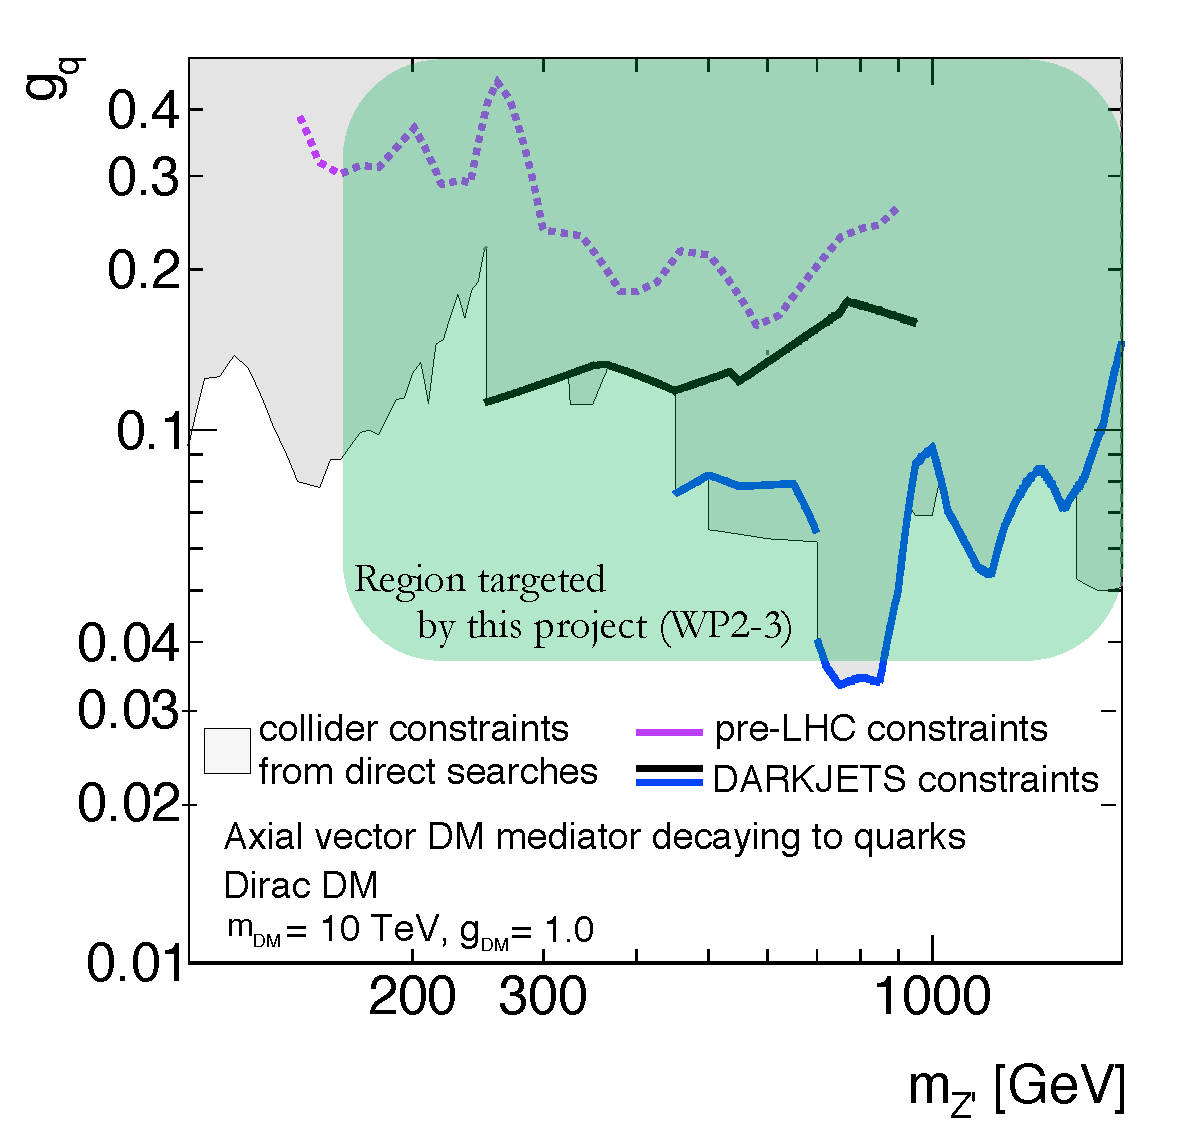
\includegraphics[width=0.45\textwidth]{figs/SummaryPlot.pdf}
\caption{Parameter space for an example  WIMP DM mediator model targeted in this project, compared to the state-of-the-art. \label{fig:pastFutureConstraints} }
\end{center}
\end{wrapfigure}

The first class of models corresponds to current benchmarks used by most LHC DM searches, a state of the art developed within my StG~\cite{Abercrombie:2015wmb,Boveia:2018yeb}. 
In these models, DM is a massive particle that interacts only weakly with SM particles---a WIMP. %AB is here 
At collider experiments, WIMPs would only weakly interact with detector material, and so they are sought traditionally by selecting events with a momentum imbalance where one or more particles has escaped detection.
WIMPs may be produced from LHC proton-proton collisions through new massive particles mediating the SM-DM interaction.
%inspired by the vector and scalar bosons that constitute the weak sector of the SM. 
This mediator would decay not only to DM particles but also into ordinary matter through the same mechanism responsible for its production.

In my StG, I delivered new searches for DM mediator decays to two quarks, leading to two sprays of collimated particles (jets) in the detector~\cite{Aaboud:2018fzt,Aaboud:2019zxd,ATLAS:2015nsi}. 
Prior to this, potential signals of mediators with masses around the crucial electroweak scale were discarded together with high-rate backgrounds from the strong force (Quantum Chromodynamics, or QCD) to meet storage constraints.
The StG search at 450--1000 GeV masses was made possible by applying the Trigger Level Analysis (TLA)\footnote{Analogue to the techniques of \textit{Data Scouting} in CMS~\cite{Khachatryan:2016ecr} and \textit{Turbo stream} in LHCb~\cite{Aaij:2016rxn}} technique to jets~\cite{Aaboud:2018fzt}. 
In the TLA technique, most of the initial data analysis and calibration is performed in real-time ($< ms$) within the ATLAS software trigger system.%, implemented in a computing farm. 
This technique records only a small amount of high-level information for further analysis, rather than the entirety of raw detector data. 
The mediator mass range between 250 and 450 GeV was covered, albeit with less sensitivity, by another new search that my colleagues and I introduced to ATLAS using traditional data taking techniques, as described below~\cite{Aaboud:2019zxd}. 
Searches using these techniques with the LHC dataset recorded from 2015 to 2018 (called \textit{Run-2}) have set some of the most stringent constraints to date for DM mediators with masses between 250 GeV and 1 TeV (see Fig.~\ref{fig:pastFutureConstraints}). 

%Mention why TLA is good here
%TODO: Ruth would like this part expanded as it is confusing
In this project, my CoG team and I will significantly extend the TLA technique beyond jets, deploying it for photons, electrons and muons for the first time to bring the greater sensitivity of the TLA approach to a larger range of mediator masses as well as to new dark matter models. 
%TODO: check that I have mentioned Run-3 trigger is new
We will validate these data-taking techniques and the new Run-3 ATLAS trigger system as a whole with physics searches and measurements in early Run-3 LHC data. 
We will subsequently exploit the full dataset containing TLA photons and jets for more sensitive and lower-mass WIMP mediator searches (see shaded yellow in Fig.~\ref{fig:pastFutureConstraints}). 
%Change wording to WAF/VR

Motivated by lack of evidence for WIMPs, the second class of models postulates interactions that are much feebler, generally involving lighter mediators. 
These models~\cite{Strassler:2006im,Cohen:2017pzm} predict a multitude of new particles in addition to the DM candidate, mirroring the complexity of the SM and similar to the strong force (\textit{dark QCD}). 
%TODO: why interesting? AB: we are checking that the kinds of sectors found in the standard model are replicated in the dark sector, e.g. dark weak sector, dark QCD sector.
Unambiguous, generic features of these models are \textit{dark jets}, which, in addition to visible particles, are comprised of invisible particles and low-mass dark matter mediators decaying into low-energy electrons and muons~\cite{Curtin:2014cca}. 
%TODO: fix optimally
Existing searches for two-jet signals are not sensitive to dark jets %, since they escape detection and are discarded at the trigger level. 
%TODO make sure that HLT computing farm is mentioned
because of the huge backgrounds from QCD processes in the SM (a problem shared by WIMP mediator searches) and because the HLT computing farm is unable to build and identify the characteristic features of dark QCD jets before the events must be discarded. 
%shorten this sentence above
To solve this problem, we will combine for the first time the TLA and the Partial Event Building (PEB) techniques. %too much??? , after extending TLA to electrons and muons
By augmenting high-level information from the data reduction in the trigger (TLA) with select raw data from detector regions around the dark jets (PEB), we will overcome the previous storage and processing limitations and enable reconstruction of the distinctive signal features at a later processing stage where more resources are available. 
We will use the dataset recorded with this technique to discover or set stringent constraints on models consistent with the DM relic density but never tested at the LHC. % explore the parameter space of dark QCD theories and
%that can fulfill the DM relic density 

As a byproduct of performing these searches, the datasets recorded with our techniques will be made available for other searches and measurements in ATLAS, extending the potential for discovery of the entire ATLAS search programme in cases where sensitivity is limited by storage constraints (e.g. low-mass leptonically-decaying DM mediators and dark sector particles~\cite{Hoenig:2014dsa}, axion-like particles~\cite{Mariotti:2017vtv}) or by HLT computing constraints (e.g. trackless jets~\cite{Daci:2015hca}).  

%TODO: rewrite coherently
Absent compelling signals of DM from any particle physics experiment, it is crucial to extract the maximum amount of information from the results obtained in these searches, and combine that information in the broader context of the global search for dark matter.
For this reason, I will continue leading the way to define community standards for LHC DM searches, 
so that any LHC discovery or constraint can be properly considered %exploited??
in synergy with complementary astroparticle, non-collider and cosmological measurements. 
Building on the success of the Dark Matter Working Group, which under my leadership set the standards for LHC WIMP search targets and for the contextualization of results alongside non-collider experiments, 
I will lead initiatives that bring together the flourishing experimental and theoretical research communities studying WIMP and non-WIMP DM scenarios~\cite{iDMEu}. 

%the impact of this proposal will not be limited to high energy physics but will be disseminated further afield to generate impact in DM direct detection and cosmological disciplines.  
% capitalizing on the information from many experiments coming online in the next decade

\section{Project organization and description} 
\smallskip


\begin{wrapfigure}{L}{0.6\textwidth} 
%\begin{figure}[h!]
\begin{center}
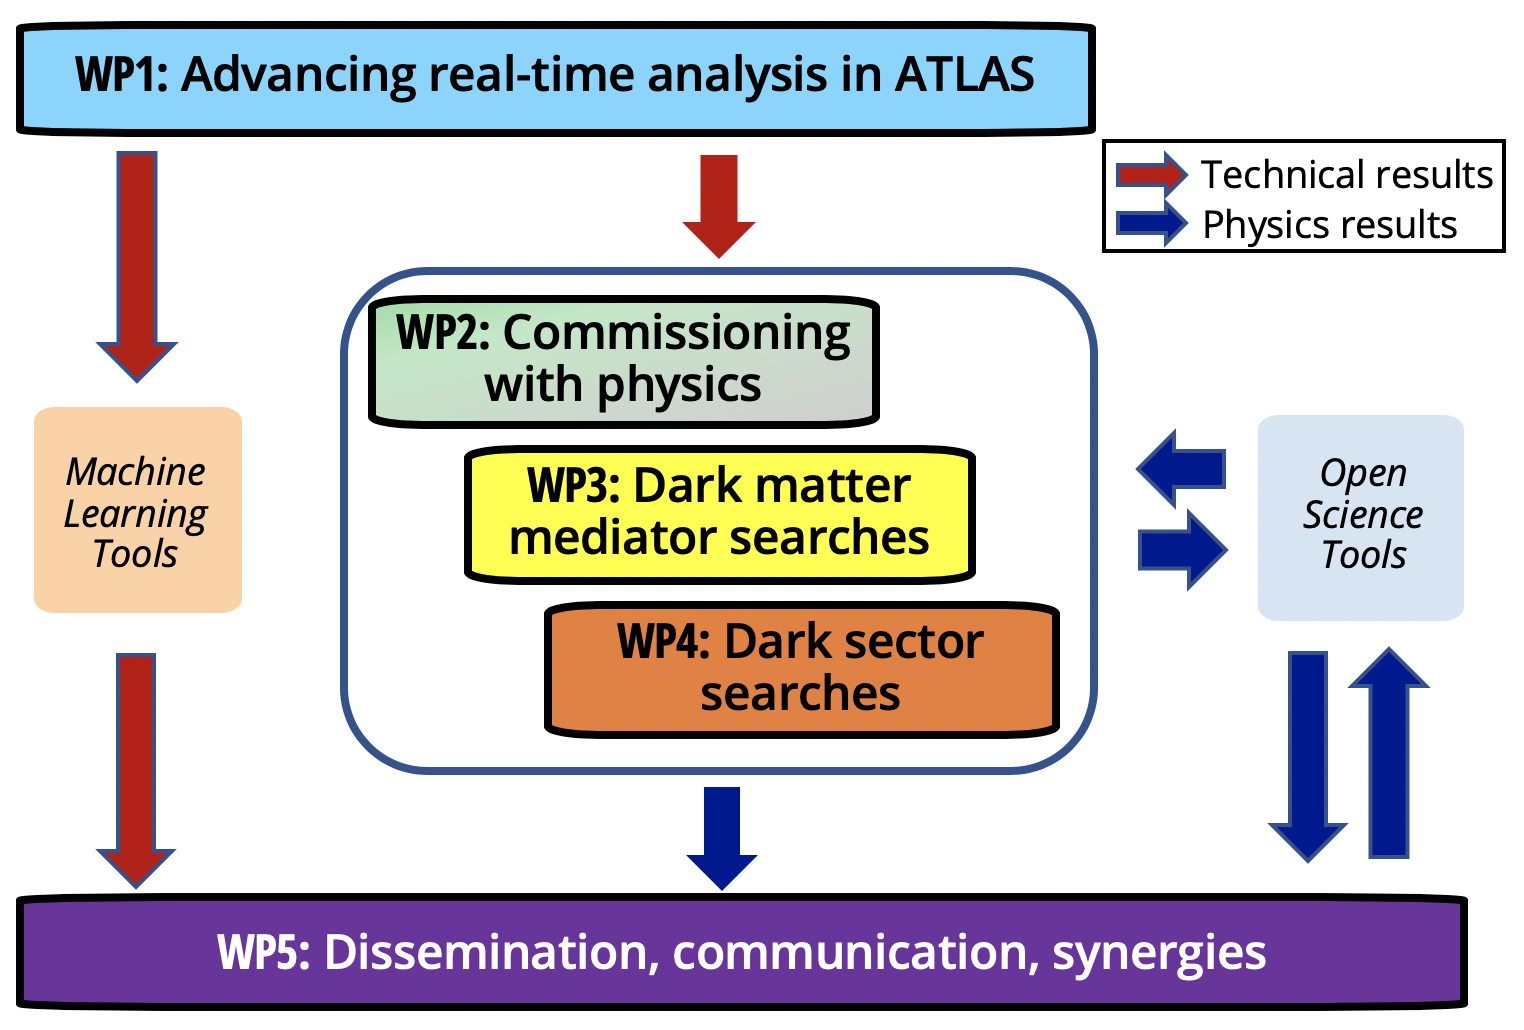
\includegraphics[width=0.6\textwidth]{figs/WPs_shorter}
\caption{\label{fig:WPs} \footnotesize Schema of work packages and expected results.
%\color{red} This will become an in-line figure, possibly on the 1st page, after feedback. If needs be, the first section will be shortened. \color{black}
}
\end{center}

\vskip10pt
\end{wrapfigure}
%\end{figure}

The project consists of five logically interconnected work packages.
%to maximise impact. 
The work packages and their interconnections are indicated in Fig.~\ref{fig:WPs}. 
In \textbf{WP1}, we will use non-standard data-taking and recording techniques to overcome key technological limitations of searches for a variety of physics phenomena including DM, as well as employ machine learning techniques for compressing data towards further gains in event storage.  
In \textbf{WP2}, we will use early physics data from Run-3 to commission the newly-upgraded ATLAS trigger system and the techniques developed in WP1.
%using physics distributions, leading to early searches and measurements.  
%TODO: Oxana/Ruth think that world-best and world-first is bragging excessively
%TODO: "dark matter models" is too generic
In \textbf{WP3 and WP4}, we will use the data recorded with the techniques developed and commissioned in WP1 and WP2 to perform world's-best and world's-first searches for dark matter models. 
In~\textbf{WP5}, we will interpret and disseminate the results of those searches, including input from LHC measurements and non-collider DM searches using Open Science tools. We will work in synergy with the broader community for optimal contextualization and dissemination of results and tools. %transgress??? Conor wants this word I don't     what is transgress, seems weird

\subsection*{\color{teal} $\blacksquare$ \color{black} WP1: Advancing real-time analysis in ATLAS}

\begin{wrapfigure}{R}{0.4\textwidth} 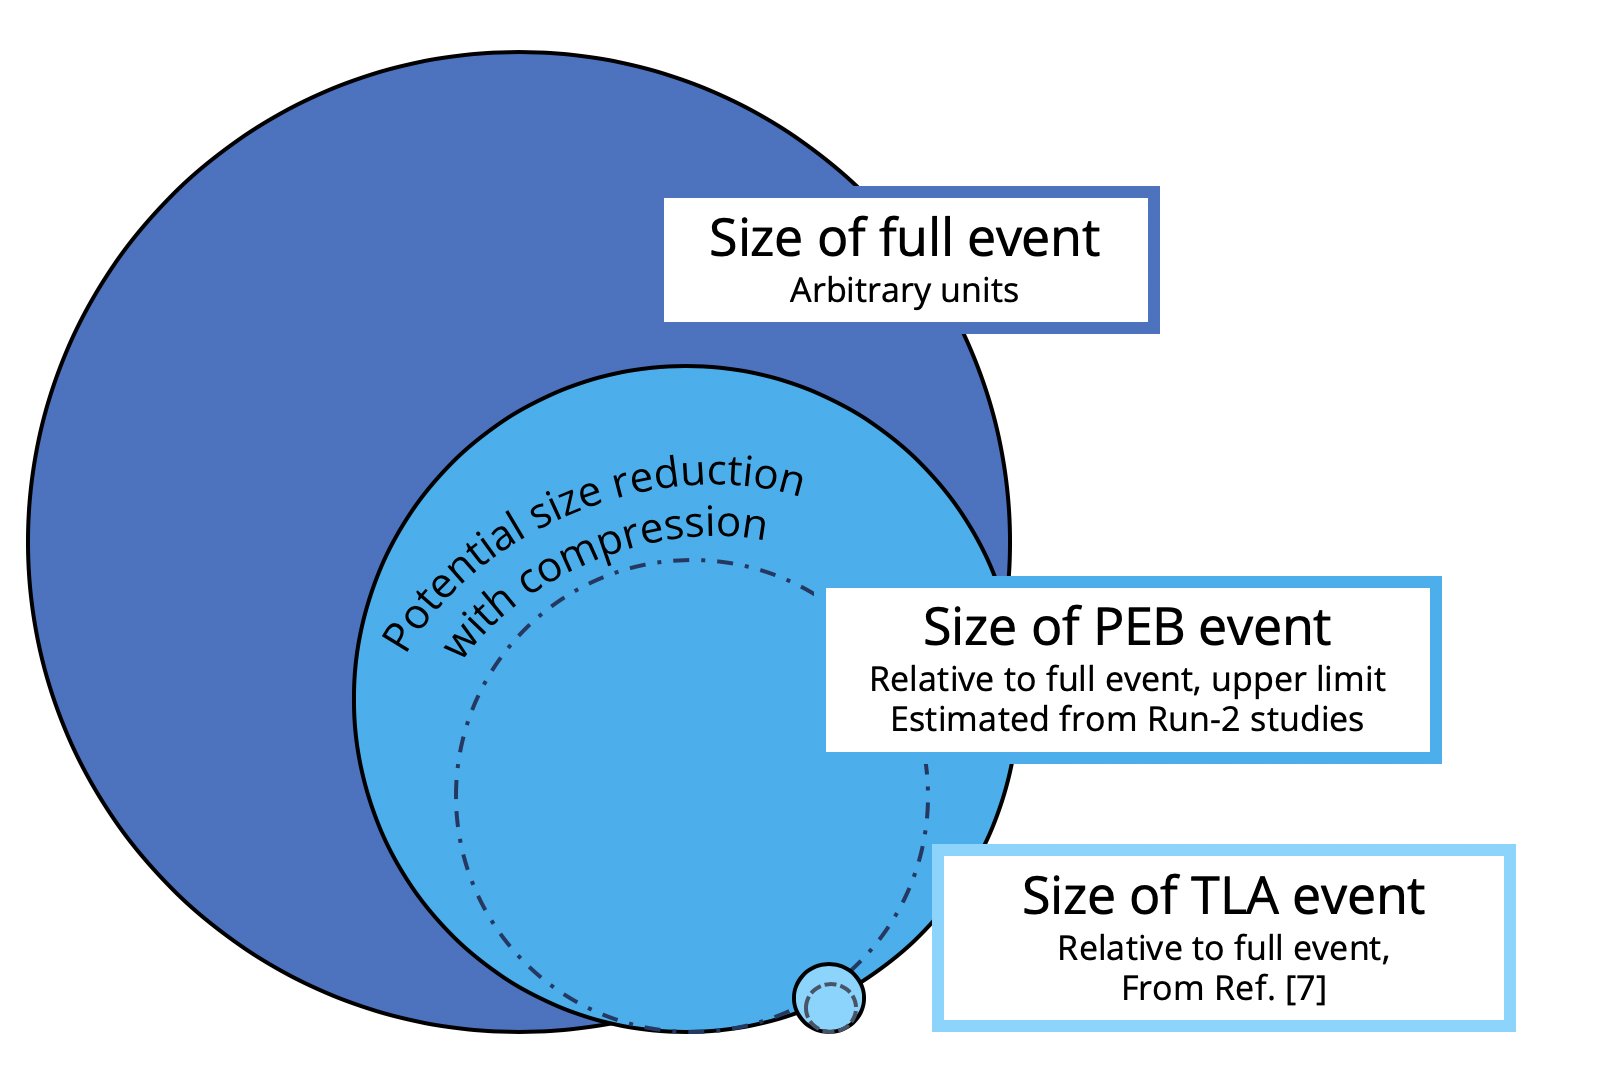
\includegraphics[width=0.4\textwidth]{figs/TLAPEB}
\caption{\label{fig:TLAPEB} \small Event sizes for traditional (full) events, and events recorded using TLA and PEB techniques~\cite{ATLASTrigger}. \scriptsize }
\end{wrapfigure}
%\color{red} If available, include estimates for this proposal. If not, change colors and only include Standard data taking and Trigger Level Analysis. Also, show how much this could be compressed if compression worked. \color{black}}

As the main technological advancement delivered by this project, we will deploy and commission the two techniques of TLA and Partial Event Building in the Run-3 trigger. 
As a pioneer of real-time analysis, I have delivered proof-of-concept studies for these techniques in my StG, but they must now be developed and commissioned on a much larger scale via WP1 in order to exploit them for groundbreaking DM searches with the Run-3 dataset.

\textbf{TLA}-recorded events contain only high-level information reconstructed in the trigger. They are considerably smaller than events with full-detector raw data, enabling the recording of a much larger number of events within the same data bandwidth.
With my StG team, I have demonstrated the effectiveness of this technique with a published proof-of-concept search for dark matter mediators decaying to jets~\cite{Aaboud:2018fzt}. 
%TODO: I already said which ones above
Within this project, I intend to expand the technique to photons, electrons and muons, allowing extensive use by ATLAS for a program of searches and measurements. 

In the \textbf{Partial Event Building} technique, high-level information available to real-time analyses is augmented by a subset of the raw detector information in selected regions of the detector. This combines the data rate enhancements of real-time analysis with the added precision of full offline reconstruction in a user-configurable manner. 
Subtle features signaling the presence of new phenomena can then be detected \textit{a posteriori}. 
This project will commission and use this technique in physics searches for the first time in ATLAS. 

Both of these techniques reduce data storage requirements with respect to traditional techniques (as shown in Fig.~\ref{fig:TLAPEB}), but they can be complemented by \textbf{further gains in data compression}. 
In this project, I will pursue a method for physics-aware data compression using using autoencoder deep neural networks~\cite{Vincent:2008:ECR:1390156.1390294,hinton}. %machine learning (ML) algorithms. 
In preliminary studies, my student and I, in collaboration with other ATLAS ML and computing experts, 
have shown the potential for an additional compression factor of two for TLA data.%, with minimal performance loss. 
This is a forward-looking activity targeting the high-luminosity LHC run in 2026 and experiments beyond the LHC.

\subsection*{\color{green} $\blacksquare$ \color{black} WP2: Commissioning the Run-3 trigger system with physics}

During the two-year shutdown between LHC Run-2 and Run-3, the ATLAS experiment trigger system is undergoing significant upgrades~\cite{Aad:1602235}, and the trigger and reconstruction software is being rewritten~\cite{Bielski:2674286}. %Stewart:2016pay
Thorough commissioning and testing is mandatory, first with simulation and cosmic ray data, and subsequently using early collision data. 
In WP2, together with my team, I \textbf{will test the completely new software trigger framework and its performance using physics quantities}.
%using the already-established TLA techniques from Run-2~\cite{Aaboud:2018fzt}.
This work will be documented by physics and technical publications.  

We will select events where at least two jets, muons or electrons are detected and reconstructed in real-time within the trigger system, and compare the performance of reconstruction and calibration between trigger-level and traditional data-taking approaches. 
%Improving the trigger-level reconstruction makes ATLAS data-taking more efficient as a whole. 
In addition to technical publications on the new software framework and its commissioning with LHC data, this WP will enable physics publications of the first Run-3 searches for low-mass DM mediators. 
We will make extensive use of the Open Science tool RECAST~\cite{Schuy:2019awp} to preserve the full analysis workflow, from detector data to final plots, so that we can take advantage of this work for the searches in WP3.  

\subsubsection*{\color{yellow} $\blacksquare$ \color{black} WP3: WIMP dark matter mediator searches}

In WP3, my team and I will \textbf{use the TLA technique to search for decays of WIMP mediators} near the crucial electroweak scale at sensitivities not possible before.
This search targets mediators with 150--350 GeV masses, a range close to where the massive mediators of the SM reside. This region is still poorly constrained, as neither traditional searches nor jet-only TLA searches have reached sensitivity to mediators with SM-like couplings (Fig.~\ref{fig:pastFutureConstraints}).  

We will employ the \textbf{dijet+ISR detector signature} that I introduced to ATLAS during Run-2 using traditional data-taking methods, where the mediator is produced in association with an additional jet or photon~\cite{Aaboud:2019zxd}. 
This approach yielded the world-leading constraint in the upper mass range of this region. 
\textbf{Performing this search with the TLA method will significantly increase its discovery potential}, 
allowing for an order of magnitude more signal events to be recorded.% and a factor \color{red}M \color{black} improvement in signal-to-background ratio. 

During the 2022-2025 grant period, we will also analyse data in the two-jet signature to search for mediators with masses above 350 GeV with the entire Run-3 dataset. 
This analysis will capitalize on the end-to-end analysis workflows set up in WP2 to make the analysis more efficient and ensure that the Run-3 results can be combined with the full Run-2 results to constrain a wide set of physics models~\cite{Kim:2019rhy}.   

\subsubsection*{\color{orange} $\blacksquare$ \color{black} WP4: Dark sector searches}

While the searches in WP3 are powerful probes of WIMPs mediated in ways inspired by the electroweak sector of the SM, they are not sensitive to dark QCD models, or to far lighter, GeV-scale DM mediators mediators whose interaction with the SM is feebler. 
For this reason, in WP4 my team and I will deploy the \textbf{combination of TLA and Partial Event Building} developed in WP1 to target this equally-compelling class of \textbf{models yielding new detector signatures}. 
WP4 focuses on two new searches.  

First, we will search for signals where DM candidates are produced in association with a large number of other dark sector particles. 
Since these dark sector particles also interact through the SM's strong force, while the DM particles escape detection, this leads to \textbf{\textit{semi-visible dark jets}}~\cite{Cohen:2017pzm}.
%Prototypes of these searches are being developed with Run-2 data, but they are limited to very high masses and to a narrow range of parameters of the model. 
We will scan a large part of the parameter space with the unique sensitivity enabled by this dataset, focusing on parameters consistent with relic density of DM~\cite{Bernreuther:2019pfb}. 

Second, we will builds on the semi-visible jet results and exploit the availability of electrons and muons at the trigger level enabled by WP1, targeting models where low-energy leptons from the decays of a light dark mediator or a dark Higgs boson are also found within dark jets~\cite{Curtin:2014cca,Falkowski:2010gv}, forming \textbf{\textit{composite  jets}}. %Cite Prestel?
This dataset will extend the ATLAS sensitivity to low-mass, low-energy and exotic objects overlooked in searches so far, which are restricted to isolated, higher-energy leptons. 

\subsubsection*{\color{violet} $\blacksquare$ \color{black} WP5: Dissemination, communication, synergies}

WP5 defines frameworks and optimal search regions in the context of the global DM search community, resulting in enhanced conceptualization and dissemination of tools and results.
This dedicated WP ensures that the results of the project have a broad research impact that exploits both local synergies and synergies with other communities. 

Within WP5, my team and I will \textbf{pinpoint the relevant parameter space} to be targeted for the new searches in WP4, and design data-taking parameters and datasets accordingly. 
%event generator = pp collision modelling?
This will be done in collaboration with the local Lund theory group, who are authors of the most widely used simulation of the models in WP4 and of the event generation software Pythia ~\cite{Sjostrand:2014zea}. 
% AB: does the following mean that you don't do a search, just reinterpret precision results?
We will use software that enables the use of precision results released by LHC collaborations~\cite{Butterworth:2016sqg}, using them for the first time to constrain dark QCD models. 

In WP5, we will ensure that all \textbf{physics results from WP2-4 are disseminated} in a way that meets the needs of other communities in terms of reproducibility, usability and complementarity in compliance with the FAIR principles~\cite{FAIR}. 
The successful experience of the Dark Matter Working Group is a stepping stone for a new, ambitious initiative that I co-founded, kicking off in Summer 2020, called \href{https://indico.cern.ch/e/iDMEu}{iDMEu}.
This initiative will permit the integration of results from this project within a much broader context that includes non-collider experiments, astrophysics, cosmology and multimessenger astronomy. 

An innovative aspect of this project is that its dissemination strategy is not limited to physics results but includes algorithms and tools. 
As I and many others advocated during the process leading to the update of the European Strategy of Particle Physics~\cite{Doglioni:2019fza}, challenges related to data acquisition, selection and analysis can be tackled more effectively and efficiently by going beyond a single experiment's boundaries. 
For this reason, WP5 also includes \textbf{sharing analysis workflows within a collaborative Dark Matter virtual environment} that I will co-lead starting from February 2020, envisaged by the \href{https://projectescape.eu}{European Science Cluster of Astronomy \& Particle physics ESFRI research infrastructures}. We will also use the \href{https://projectescape.eu/services/open-source-scientific-software-and-service-repository}{ESCAPE Software Repository} to \textbf{share generic data reduction software and data compression algorithms} with other experiments where a reduced storage footprint is necessary to increase the physics potential within the same computing resources. %, such as gravitational wave experiments \color{red}~\cite{GravWavesCompression}\color{black}. 

\section{Timeliness and timeline of the research program} 
\smallskip

I will lead a research team of two postdoctoral researchers and two graduate students, working on the two lines of physics analysis in this project, and frequently collaborating to share technical tasks and software. An additional software engineer will augment the team during the demanding time of the LHC Run-3 startup. 
For WP1, the team will be joined by talented Lund University undergraduates that I have a track record of recruiting and training who will work on the forward-looking ML compression activities.
The research program spans the entire upcoming Run-3 LHC data-taking period.
%and its timeline is shown in Fig.~\ref{fig:timeline}. 
The 2021-2026 period is the ideal time to advance the state-of-the-art in processing of large datasets and DM searches, as it ensures continued impact through a significant extension of my current successful StG research program that pioneered proof-of-principle real-time searches in ATLAS. 
The current LHC schedule includes an initial commissioning period where innovations can be deployed and tested via early measurements with Run-3 start-up data, which forms the first part of this project (WP1 and WP2), readying them for the second phase of the project where the LHC will be in production mode.   
The second (WP3 and WP4) phase of this project will exploit the wealth of LHC data delivered by WP1 and WP2 for novel DM searches, with a dataset that will be much more sensitive to the models sought in this project than the data collected so far. 
Throughout the timeline of entire project, in WP5 we will share tools and results within the global DM community, to answer one of the most pressing questions of our universe with a discovery or by defining future search directions in which such a discovery will be made. 

%TODO: Ruth suggests to have a plan B?

%contextualize the results of the searches in this proposal and the LHC research program within
%The team will start with commissioning the techniques in WP1 (2021) as the the students fulfill their authorship qualification tasks in the trigger system. 
%The jet and photon TLA techniques will be ready in coincidence with early data taking in Summer 2021, while the delivery of TLA muons and electrons is planned for mid-2022. 
%Partial Event Building will also be commissioned with 2022 data, and the second

% Mention who asked you to do this rather than saying who you're doing this with
%In addition to further enhancing my standing as an expert in DM, 

%As a recognized expert in DM searches and collider data taking techniques with a track record of synergistic interdisciplinary activities, the impact of this proposal will not be limited to high energy physics but will be 
\clearpage

\setboolean{inbibliography}{true}
\bibliographystyle{JHEP}
\bibliography{researchrefs}

{\bf Note:} The PI is the editor of Refs.~\cite{Boveia:2018yeb,Abercrombie:2015wmb,Aaboud:2018fzt,Aaboud:2019zxd,Doglioni:2019fza}, the initiator of the activities in Refs.~\cite{DMWGWebsite,iDMEu} and has made significant contributions to Refs.~\cite{Strategy:2019vxc,Alves:2017she,Aaboud:2016leb,Aaboud:2019yqu}. The PI is the author of all publications by the ATLAS collaboration.
% -- Refs.~\cite{Alves:2008zz,CERN-LHCC-2014-016,LHCb:2011aa,Aaij:2013mga,Aaij:2014ywt}.
%The PI is the contact author within LHCb for Ref.~\cite{Aaij:2014ywt}.

\end{document}